\subsection{Module}
De module is de Haskell bibliotheek die de programmeur gebruikt om de grafische interface in de client te bedienen. Naar de programmeur is de gebruiksvriendelijkheid van de biblotheek een van de belangrijkste overwegingen voor het ontwerp. De module bestaat uit een aantal onderdelen: de server die de statische bestanden serveert, de websocket server die de verbinding met de client onderhoud, en de laag die de input en output verwerkt. \autoref{fig:architecture_module} geeft de architectuur weer van de module.

-TODO: Ontwerpkeuze toelichten: unsafePerformIO in Server.hs

\begin{figure}
\begin{center}
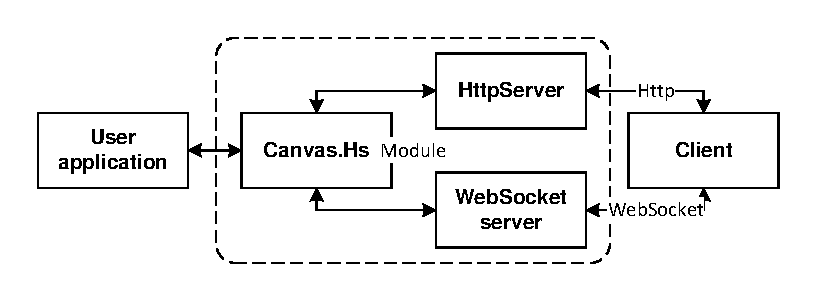
\includegraphics[keepaspectratio,width=\textwidth]{./images/module_architecture.pdf}
\caption{Architectuur van de module}
\label{fig:architecture_module}
\end{center}
\end{figure}

\paragraph{Servers}
Canvas.hs draait een simpele server op port 80 die statische bestanden kan serveren. Waaronder de index pagina, de javascript bestanden en eventueel plaatjes. Op port 8080 draait een websocket server die de verbinding met de client onderhoud.


\paragraph{Server in de module}
De server draait in het process wat gestart wordt vanuit de Haskell-code van de programmeur. De main van de programmeur start (indirect) de server. Dit is envoudiger dan het draaien van de server in een apart process. Er hoeft namelijk niet tussen verschillende Haskell-processen gecommuniceerd te worden. Dit scheelt het schrijven van nog een interface tussen het server- en het module process. Nadeel is wel dat het voortdurend opnieuw starten en afsluiten van de server leidt tot vertraging in het opstarten van het programma van de programmeur. Dit is vervelend als de programmeur regelmatig kleine wijzigingen maakt en dan de code opnieuw moet starten. Echter lijkt de overhead van het opnieuw starten van de server minimaal. Het is verder praktisch dat er geen rekening gehouden hoeft te worden met de state van de server bij het opstarten van het programma.

\paragraph{Gebruik} Wanneer de programmeur gebruik wil maken van de Canvas.hs moet hij gebruik maken van de installEventHandler functie. Bij het aanroepen van deze functie moet de programmeur een event handler meegeven die alle events vanuit de interface afhandeld. Om het gebruik van Canvas.hs zo makkelijk mogelijk te houden zal bij het aanroepen van installEventHandler automatisch de statische server en de websocket server gestart worden, en daarna automatisch de browserpagina geopend worden. \autoref{fig:startup_procedure} geeft de opstartprocedure weer.

\begin{figure}
\begin{center}
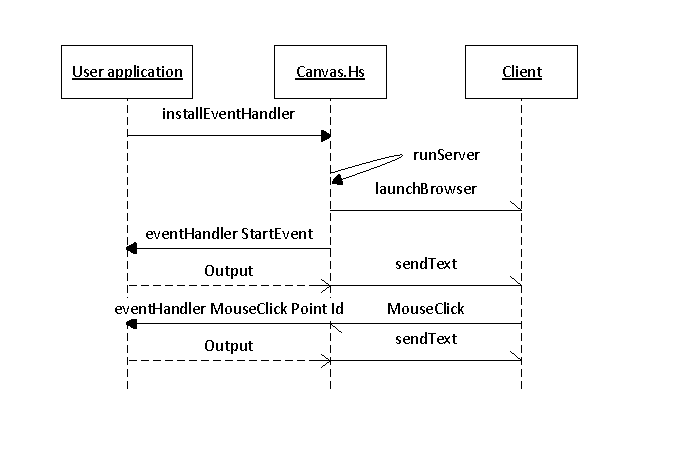
\includegraphics[keepaspectratio,width=\textwidth]{./images/module_startup_procedure_interaction.pdf}
\caption{De opstartprocedure en initiele interactiesequentie}
\label{fig:startup_procedure}
\end{center}
\end{figure}

\paragraph{Input/output}
De module handeld input en output af door events naar de eventhandler van de programmeur te sturen. Bijvoorbeeld: wanneer een gebruiker op een rondje klikt zal het programma de event handler aanroepen met de ID van dat rondje en de lokatie van de muisklik. De event handler van de programmeur kan dan nieuwe output genereren op basis van dit event. Zoals een nieuw menu weergeven of het uitvoeren van een actie zoals het opvragen van een bestand van de gebruiker.In \autoref{fig:startup_procedure} is deze interactie weergegeven. 

\paragraph{Unsafe I/O}
In Server.hs wordt gebruik gemaakt van unsafePreformIO voor het starten van child processen (een MVar die threads bijhoudt) en om een verbinding met een client bij te houden (een IORef die de connections naar de clients bevat). Hoewel het in dit geval volkomen veilig is, zijn er bezwaren tegen het gebruik van unsafePerformIO\cite{Haskell.org2008}. Dit is namelijk niet de netste oplossing en kan meestal voorkomen worden. Het is netter om een Server Monad te gebruiken die een State implementeert die deze zaken bijhoudt. Echter is het implementeren daarvan tijdsintensief, waardoor voor deze oplossing is gekozen.